%-------------------------------------------------------------------------------
% DEFINITIONS
%-------------------------------------------------------------------------------
\subsection{Définition du problème}

% LEFT-HAND SIDE
\begin{minipage}[b]{0.3\linewidth}
\centering
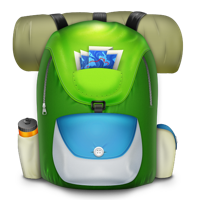
\includegraphics[height=3cm]{../images/Knapsack.png}
\end{minipage}
% RIGHT-HAND SIDE
\hspace{0.5cm}
\begin{minipage}[b]{0.7\linewidth}
Le problème de Sac à Dos, ou \og Knapsack \fg{} en Anglais, s'énonce
de la manière suivante : nous avons un ensemble d'objets ayant chacun
un poids (respectivement, un volume) et une valeur d'utilité. Nous
devions choisir parmi ces objets un sous-ensemble dont le poids
(respectivement volume) total ne dépasse pas un certain seuil (la
capacité de notre sac), mais de telle manière que l'utilité totale
soit maximisée.
\end{minipage}

Ce problème se modélise en programmation linéaire de la manière
suivante, où b est la capacité du sac, $c_i$ l'utilité et $a_i$ de
l'objet i, et $x_i = 1$ si l'objet i est prise et $0$ sinon ~:

\begin{equation}
\begin{cases}
Max~z=\sum_{i=1}^nc_ix_i \\
\sum_{i=1}^na_ix_i \leq b \\
x_i \in\{0, 1\}, i=1\dots n\\
\end{cases}
\end{equation}

Le problème de Sac à Dos apparaît souvent dans le réel : il existe un
grand nombre d'applications économiques (ex: choix d'investissements)
et industrielles (ex: découpage de minerai).

%-------------------------------------------------------------------------------
% NOTATIONS
%-------------------------------------------------------------------------------
\subsection{Notations}

Par la suite nous utiliserons les notations suivantes :

\begin{itemize}
\item \textbf{P} : la capacité maximum de notre sac,
\item \textbf{n} : le nombre d'objet,
\item \textbf{poids[i]} : le poids de la $i^{i+1\grave{e}me}$ objet,
\item \textbf{utilité[i]} : l'utilité de la $i^{i+1\grave{e}me}$ objet,
\item \textbf{optimale[i][p]} : l'utilité maximum atteignable en utilisant les $i$ premières objets et en respectant un poids totale de $p$.
\end{itemize} 

Nous cherchons à connaître optimale[n][P]. Nous verrons par la suite
qu'il est possible de calculer cette valeur à partir de
optimale[n-1][P] et optimale[n-1][P-poids[i]], et caetera de manière
récursive.

%-------------------------------------------------------------------------------
% FORMULAS
%-------------------------------------------------------------------------------
\subsection{Formule de récurrence}
Nous construisons un tableau de résultats intermédiaires ligne par
ligne et colonne par colonne. La première ligne du tableau est remplie
à la main : évidement l'utilité maximum n'est atteignable qu'avec
l'objet $0$ et sa propre utilité, sous réserve que le poids que nous
nous permettons est au-dessus de $poids[0]$. Ainsi nous arrivons à
l'équation \ref{knapsack_rec}.

\begin{equation}
\label{knapsack_rec}
optimale[0][p] =
	\begin{cases}
		0 \text{ si } p < poids[0];	\\
		utilit\acute{e}[i] \text{ sinon};
	\end{cases} \\
\end{equation}

Si nous ne prenons pas l'objet $i$ alors nous n'augmentons pas
l'utilité maximum par rapport au maximum atteignable avec l'ensemble
des objets $0 \dots i-1$. Nous définissons alors l'utilité maximale en
laissant l'objet $i$ avec l'équation \ref{laisser}.

\begin{equation}
\label{laisser}
laisser(i, p) = optimale[i-1][p];
\end{equation}


Si par contre l'objet $i$ est pris, il faut s'assurer qu'il y ait de
la place pour lui, donc nous ajoutons son utilité à l'utilité maximum
atteignable avec les objets $0 \dots i-1$ et un poids inférieur ou
égal à $p-poids[i]$. Ainsi l'utilité maximale si nous prenons l'objet
$i$ est décrite par l'équation \ref{prendre}.

\begin{equation}
\label{prendre}
prendre(i, p) = optimale.t[i-1][p - poids[i]] + utilit\acute{e}[obj];
\end{equation}

Nous pouvons finalement remplir notre tableau de manière récursive, pour $i \neq 0$, en utilisant l'équation \ref{prendre_ou_laisser}.

\begin{equation}
\label{prendre_ou_laisser}
optimale[i][p] =
	\begin{cases}
		laisser(i, p) \text{ si } p < poids[i];	\\
		max(prendre(i, p), laisser(i, p)) \text{ sinon};
	\end{cases}
\end{equation}


%-------------------------------------------------------------------------------
% ALGORITHME
%-------------------------------------------------------------------------------
\subsection{Algorithme}

Nous pouvons finalement proposer l'algorithme \ref{dp_knapsack}.

\begin{algorithm}[!ht]
\caption{DP Knapsack}
\label{dp_knapsack}
\begin{algorithmic}[1]
\REQUIRE maximum capacity $W$, number of objects $n$, $weights[n]$, $utilities[n]$  
\FOR{$w$ from 1 to $W$}
	\IF{weights[0] $\leq$ w }
		\STATE $optimal[0][w] := utilities[0]$
	\ENDIF
\ENDFOR
\FOR{$w$ from 1 to $n$}
	\FOR{$w$ from 1 to $W$}
		\STATE leave := optimal[i-1][w]
		\STATE take := optimal[i-1][w-weights[i]] + utilities[i]
		\IF{weights[i] $\leq$ w }
			\STATE $optimal[i][w] := max(leave, take)$
		\ELSE
			\STATE $optimal[i][w] := leave$
		\ENDIF
	\ENDFOR
\ENDFOR
\RETURN optimal[n][W]
\end{algorithmic}
\end{algorithm}

Étant donné que cet algorithme itère sur les poids et les objets, la
complexité temporelle est de $O(nW)$. Il en va de même pour sa
complexité mémoire.

À noter que la topologie du tableau finale nous permet en plus de connaitre l'utilité optimal de connaitre l'ensemble des objets prises en partant de la dernière case et en remontant vers le haut et la gauche. Il est possible donc de restituer un certificat en plus d'une réponse.

%-------------------------------------------------------------------------------
% IMPLEMENTATION
%-------------------------------------------------------------------------------
\subsubsection{Implémentation en \texttt{C}}
Une fois énoncé, l'algorithme est simple à implémenter. Nous nous
basons sur notre propre structure de matrice \texttt{matrix\_t}:

\lstinputlisting[language=C,morekeywords={}]{../code/knapsack.c} 


%-------------------------------------------------------------------------------
% TESTS
%-------------------------------------------------------------------------------
\subsection{Tests et conclusion}

Pour vérifier que notre implémentation respecte bien la complexité théorique de $O(nW)$ nous avons lancé une batterie des tests en faisant varier : 

\begin{itemize}
\item le nombre d'objets, avec la capacité fixé à $5000$,
\item la capacité, avec un nombre d'objets fixé à $100$.
\end{itemize}

Les valeurs rapportées dans les figures \ref{knapsack_test_objects} et
\ref{knapsack_test_capacity} sont des temps moyens d'exécution pour
$100$ tests. Le poids et l'utilité de chaque objet sont générés
aléatoirement, mais les poids sont bornés par la capacité (aucun
élément n'est jamais plus grand que le sac entier).

\begin{figure}[ht]
% LEFT-HAND SIDE
\begin{minipage}[b]{0.5\linewidth}
\centering
\begin{tikzpicture}[scale=0.9]
    \begin{axis}[title=Variation du nombre d'objets, xlabel= nombre d'objets, ylabel= temps d'exécution]
      \addplot
        table[col sep=comma]{../charts/sac.csv};
        %\legend{exécution de sac à dos}
    \end{axis}
\end{tikzpicture}
\caption{Temps d'exécution de Sac à Dos avec nombre d'objets variable.}
\label{knapsack_test_objects}
\end{minipage}
% RIGHT-HAND SIDE
\hspace{0.5cm}
\begin{minipage}[b]{0.5\linewidth}
\centering
\begin{tikzpicture}[scale=0.9]
    \begin{axis}[title=Variation de la capacité, xlabel= capacité, ylabel= temps d'exécution]
      \addplot
        table[col sep=comma]{../charts/sac1.csv};
        %\legend{exécution de Sac à Dos}
    \end{axis}
\end{tikzpicture}
\caption{Temps d'exécution de Sac à Dos avec capacité variable.}
\label{knapsack_test_capacity}
\end{minipage}
\end{figure}

Notre implémentation est clairement linéaire en le nombre d'objets et
la capacité maximum, ce qui correspond bien à la complexité théorique.
